\documentclass[11pt]{article}

% Related to page geometry
\usepackage[a4paper,vmargin={2.4cm,2.4cm},hmargin={2.4cm,2.4cm}]{geometry}
\usepackage[utf8]{inputenc}
\usepackage{amsmath}
\usepackage{caption}
\usepackage{graphicx}
\usepackage{float}

\author{}
\title{Report on Cooperative Optimization Project}
\date{March 2026}

\begin{document}

\maketitle

\section{Part I}
\subsection{Decentralized gradient descent and gradient tracking}
\subsubsection{Justification of the step size}
Let denote the agent $A_1, A_2, \dots, A_5$
The function $f_i$ for each agent is:
\begin{equation}
    f_i(\alpha)=\dfrac{\sigma^2}{5}\dfrac{1}{2}\alpha^T K_{mm}\alpha+\dfrac{1}{2}\sum_{i\in A_i}(y_i-K_{(i)m}\alpha)^2+\dfrac{\nu}{10}\lVert \alpha \rVert^2
\end{equation}
One has:
\begin{equation}
    \nabla_{\alpha}f_i(\alpha)=\dfrac{\sigma^2}{5}K_{mm}\alpha-\sum_{i\in A_i}K_{(i)m}^T(y_i-K_{(i)m}\alpha) +\dfrac{\nu}{5}\alpha
\end{equation}
Then:
\begin{equation}
\nabla_{\alpha}^2f_i(\alpha)=\dfrac{\sigma^2}{5}K_{mm} + \sum_{i\in A_i} K_{(i)m}^T K_{(i)m}+\dfrac{\nu}{5}I_m
\end{equation}So, let $\lambda_{i, \text{max}} = \arg\max_{\lambda \in \mathrm{Sp}\big(\nabla_{\alpha}^2 f_i(\alpha)\big)} |\lambda|$ for each agent $i$. Let $L=\max_i{|\lambda_{i, \text{max}}}|$. Then, we need to choose a step size which fulfilled is $\leq O\left(\dfrac{1}{L}\right)$.
\subsubsection{Plot convergence depending on graph structure}
\begin{figure}[!h]
    \centering
    \includegraphics[width=0.8\textwidth]{Figures/DGD_GT_Fully_connected.pdf}
    \caption{Convergence in terms of $\lVert \alpha_i-\alpha^*\rVert$ for DGD and Gradient tracking on the Kernel ridge example for a fully connected graph.}
\end{figure}

\begin{figure}[!h]
    \centering
    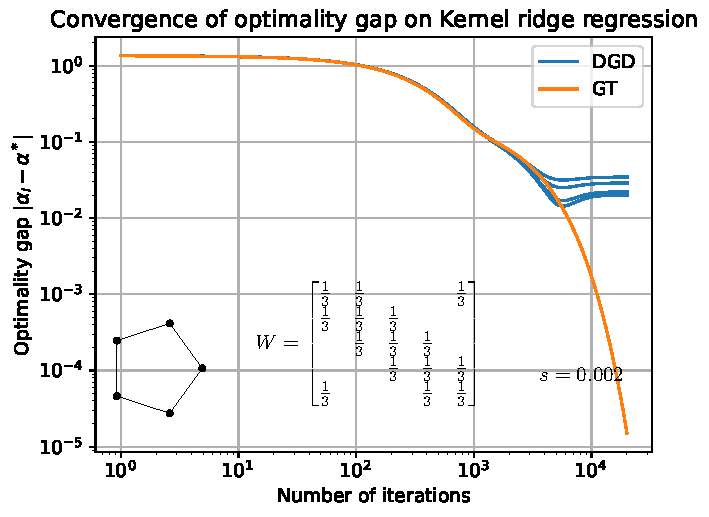
\includegraphics[width=0.8\textwidth]{Figures/DGD_GT_small_world.pdf}
    \caption{Convergence in terms of $\lVert \alpha_i-\alpha^*\rVert$ for DGD and Gradient tracking on the Kernel ridge example for a small world graph.}
\end{figure}

\begin{figure}[!h]
    \centering
    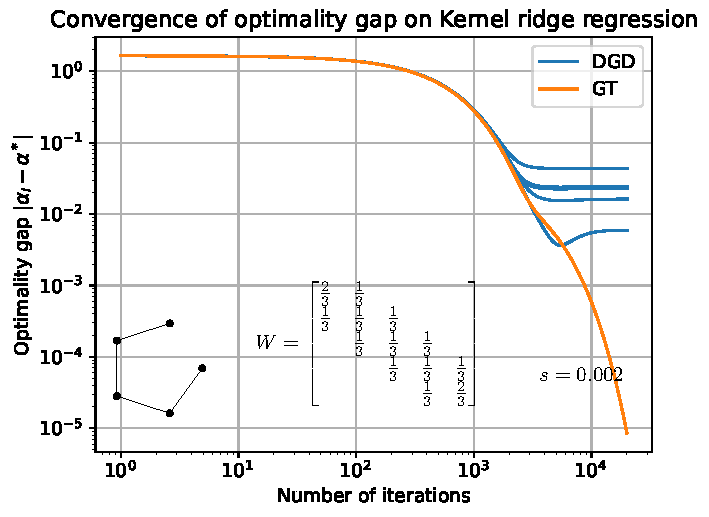
\includegraphics[width=0.8\textwidth]{Figures/DGD_GT_line.pdf}
    \caption{Convergence in terms of $\lVert \alpha_i-\alpha^*\rVert$ for DGD and Gradient tracking on the Kernel ridge example for a line graph.}
\end{figure}

Concerning the DGD, we observe the smaller is the error ball, and the better is the consensus. 
Indeed, one has theoticaly, that the error ball for DGD is of order $O\left(\dfrac{\alpha}{1-\gamma}\right)$ where $\gamma$ is the spectral gap of the graph, and $\alpha$ is the step size.
We also have an error on the consensus, which is of order $O\left(\dfrac{\alpha}{1-\gamma}\right)$.
The gradient tracking algorithm it reaches zero error ball and zero consensus error.

\subsubsection{Visualization of the obtained function}
test
\end{document}
